\documentclass[english, 11 pt, class=article, crop=false]{standalone}

% note
\newcommand{\note}{Note}
\newcommand{\notesm}[1]{{\footnotesize \textsl{\note:} #1}}
\newcommand{\selos}{See the solutions manual.}

\newcommand{\texandasy}{The text is written in \LaTeX\ and the figures are made with the aid of Asymptote.}

\newcommand{\ekstitle}{Example }
\newcommand{\sprtitle}{The language box}
\newcommand{\expl}{explanation}

%%% SECTION HEADLINES %%%

% Our numbers
\newcommand{\likteikn}{The equal sign}
\newcommand{\talsifverd}{Numbers, digits and values}
\newcommand{\koordsys}{Coordinate systems}

% Calculations
\newcommand{\adi}{Addition}
\newcommand{\sub}{Subtraction}
\newcommand{\gong}{Multiplication}
\newcommand{\del}{Division}

%Factorization and order of operations
\newcommand{\fak}{Factorization}
\newcommand{\rrek}{Order of operations}

%Fractions
\newcommand{\brgrpr}{Introduction}
\newcommand{\brvu}{Values, expanding and simplifying}
\newcommand{\bradsub}{Addition and subtraction}
\newcommand{\brgngheil}{Fractions multiplied by integers}
\newcommand{\brdelheil}{Fractions divided by integers}
\newcommand{\brgngbr}{Fractions multiplied by fractions}
\newcommand{\brkans}{Cancelation of fractions}
\newcommand{\brdelmbr}{Division by fractions}
\newcommand{\Rasjtal}{Rational numbers}

%Negative numbers
\newcommand{\negintro}{Introduction}
\newcommand{\negrekn}{The elementary operations}
\newcommand{\negmeng}{Negative numbers as amounts}

%Calculation methods
\newcommand{\delmedtihundre}{Deling med 10, 100, 1\,000 osv.}

% Geometry 1
\newcommand{\omgr}{Terms}
\newcommand{\eignsk}{Attributes of triangles and quadrilaterals}
\newcommand{\omkr}{Perimeter}
\newcommand{\area}{Area}

%Algebra 
\newcommand{\algintro}{Introduction}
\newcommand{\pot}{Powers}
\newcommand{\irrasj}{Irrational numbers}

%Equations
\newcommand{\ligintro}{Introduction}
\newcommand{\liglos}{Solving with the elementary operations}
\newcommand{\ligloso}{Solving with elementary operations summarized}

%Functions
\newcommand{\fintro}{Introduction}
\newcommand{\lingraf}{Linear functions and graphs}

%Geometry 2
\newcommand{\geoform}{Formulas of area and perimeter}
\newcommand{\kongogsim}{Congruent and similar triangles}
\newcommand{\geofork}{Explanations}

% Names of rules
\newcommand{\adkom}{Addition is commutative}
\newcommand{\gangkom}{Multiplication is commutative}
\newcommand{\brdef}{Fractions as rewriting of division}
\newcommand{\brtbr}{Fractions multiplied by fractions}
\newcommand{\delmbr}{Fractions divided by fractions}
\newcommand{\gangpar}{Distributive law}
\newcommand{\gangparsam}{Paranthesis multiplied together}
\newcommand{\gangmnegto}{Multiplication by negative numbers I}
\newcommand{\gangmnegtre}{Multiplication by negative numbers II}
\newcommand{\konsttre}{Unique construction of triangles}
\newcommand{\kongtre}{Congruent triangles}
\newcommand{\topv}{Vertical angles}
\newcommand{\trisum}{The sum of angles in a triangle}
\newcommand{\firsum}{The sum of angles in a quadrilateral}
\newcommand{\potgang}{Multiplication by powers}
\newcommand{\potdivpot}{Division by powers}
\newcommand{\potanull}{The special case of \boldmath $a^0$}
\newcommand{\potneg}{Powers with negative exponents}
\newcommand{\potbr}{Fractions as base}
\newcommand{\faktgr}{Factors as base}
\newcommand{\potsomgrunn}{Powers as base}
\newcommand{\arsirk}{The area of a circle}
\newcommand{\artrap}{The area of a trapezoid}
\newcommand{\arpar}{The area of a parallelogram}
\newcommand{\pyt}{Pythagoras's theorem}
\newcommand{\forform}{Ratios in similar triangles}
\newcommand{\vilkform}{Terms of similar triangles}
\newcommand{\omkrsirk}{The perimeter of a circle (and the value of $ \bm \pi $)}
\newcommand{\artri}{The area of a triangle}
\newcommand{\arrekt}{The area of a rectangle}
\newcommand{\liknflyt}{Moving terms across the equal sign}
\newcommand{\funklin}{Linear functions}


\usepackage[T1]{fontenc}
%\renewcommand*\familydefault{\sfdefault} % For dyslexia-friendly text
\usepackage{lmodern} % load a font with all the characters
\usepackage{geometry}
\geometry{verbose,paperwidth=16.1 cm, paperheight=24 cm, inner=2.3cm, outer=1.8 cm, bmargin=2cm, tmargin=1.8cm}
\setlength{\parindent}{0bp}
\usepackage{import}
\usepackage[subpreambles=false]{standalone}
\usepackage{amsmath}
\usepackage{amssymb}
\usepackage{esint}
\usepackage{babel}
\usepackage{tabu}
\makeatother
\makeatletter

\usepackage{titlesec}
\usepackage{ragged2e}
\RaggedRight
\raggedbottom
\frenchspacing

% Norwegian names of figures, chapters, parts and content
\addto\captionsenglish{\renewcommand{\figurename}{Figur}}
\makeatletter
\addto\captionsenglish{\renewcommand{\chaptername}{Kapittel}}
\addto\captionsenglish{\renewcommand{\partname}{Del}}


\usepackage{graphicx}
\usepackage{float}
\usepackage{subfig}
\usepackage{placeins}
\usepackage{cancel}
\usepackage{framed}
\usepackage{wrapfig}
\usepackage[subfigure]{tocloft}
\usepackage[font=footnotesize,labelfont=sl]{caption} % Figure caption
\usepackage{bm}
\usepackage[dvipsnames, table]{xcolor}
\definecolor{shadecolor}{rgb}{0.105469, 0.613281, 1}
\colorlet{shadecolor}{Emerald!15} 
\usepackage{icomma}
\makeatother
\usepackage[many]{tcolorbox}
\usepackage{multicol}
\usepackage{stackengine}

\usepackage{esvect} %For vectors with capital letters

% For tabular
\usepackage{array}
\usepackage{multirow}
\usepackage{longtable} %breakable table

% Ligningsreferanser
\usepackage{mathtools}
\mathtoolsset{showonlyrefs}

% index
\usepackage{imakeidx}
\makeindex[title=Indeks]

%Footnote:
\usepackage[bottom, hang, flushmargin]{footmisc}
\usepackage{perpage} 
\MakePerPage{footnote}
\addtolength{\footnotesep}{2mm}
\renewcommand{\thefootnote}{\arabic{footnote}}
\renewcommand\footnoterule{\rule{\linewidth}{0.4pt}}
\renewcommand{\thempfootnote}{\arabic{mpfootnote}}

%colors
\definecolor{c1}{cmyk}{0,0.5,1,0}
\definecolor{c2}{cmyk}{1,0.25,1,0}
\definecolor{n3}{cmyk}{1,0.,1,0}
\definecolor{neg}{cmyk}{1,0.,0.,0}

% Lister med bokstavar
\usepackage[inline]{enumitem}

\newcounter{rg}
\numberwithin{rg}{chapter}
\newcommand{\reg}[2][]{\begin{tcolorbox}[boxrule=0.3 mm,arc=0mm,colback=blue!3] {\refstepcounter{rg}\phantomsection \large \textbf{\therg \;#1} \vspace{5 pt}}\newline #2  \end{tcolorbox}\vspace{-5pt}}

\newcommand\alg[1]{\begin{align} #1 \end{align}}

\newcommand\eks[2][]{\begin{tcolorbox}[boxrule=0.3 mm,arc=0mm,enhanced jigsaw,breakable,colback=green!3] {\large \textbf{Eksempel #1} \vspace{5 pt}\\} #2 \end{tcolorbox}\vspace{-5pt} }

\newcommand{\st}[1]{\begin{tcolorbox}[boxrule=0.0 mm,arc=0mm,enhanced jigsaw,breakable,colback=yellow!12]{ #1} \end{tcolorbox}}

\newcommand{\spr}[1]{\begin{tcolorbox}[boxrule=0.3 mm,arc=0mm,enhanced jigsaw,breakable,colback=yellow!7] {\large \textbf{Språkboksen} \vspace{5 pt}\\} #1 \end{tcolorbox}\vspace{-5pt} }

\newcommand{\sym}[1]{\colorbox{blue!15}{#1}}

\newcommand{\info}[2]{\begin{tcolorbox}[boxrule=0.3 mm,arc=0mm,enhanced jigsaw,breakable,colback=cyan!6] {\large \textbf{#1} \vspace{5 pt}\\} #2 \end{tcolorbox}\vspace{-5pt} }

\newcommand\algv[1]{\vspace{-11 pt}\begin{align*} #1 \end{align*}}

\newcommand{\regv}{\vspace{5pt}}
\newcommand{\mer}{\textsl{Merk}: }
\newcommand{\mers}[1]{{\footnotesize \mer #1}}
\newcommand\vsk{\vspace{11pt}}
\newcommand\vs{\vspace{-11pt}}
\newcommand\vsb{\vspace{-16pt}}
\newcommand\sv{\vsk \textbf{Svar} \vspace{4 pt}\\}
\newcommand\br{\\[5 pt]}
\newcommand{\figp}[1]{../fig/#1}
\newcommand\algvv[1]{\vs\vs\begin{align*} #1 \end{align*}}
\newcommand{\y}[1]{$ {#1} $}
\newcommand{\os}{\\[5 pt]}
\newcommand{\prbxl}[2]{
\parbox[l][][l]{#1\linewidth}{#2
	}}
\newcommand{\prbxr}[2]{\parbox[r][][l]{#1\linewidth}{
		\setlength{\abovedisplayskip}{5pt}
		\setlength{\belowdisplayskip}{5pt}	
		\setlength{\abovedisplayshortskip}{0pt}
		\setlength{\belowdisplayshortskip}{0pt} 
		\begin{shaded}
			\footnotesize	#2 \end{shaded}}}

\renewcommand{\cfttoctitlefont}{\Large\bfseries}
\setlength{\cftaftertoctitleskip}{0 pt}
\setlength{\cftbeforetoctitleskip}{0 pt}

\newcommand{\bs}{\\[3pt]}
\newcommand{\vn}{\\[6pt]}
\newcommand{\fig}[1]{\begin{figure}
		\centering
		\includegraphics[]{\figp{#1}}
\end{figure}}

\newcommand{\figc}[2]{\begin{figure}
		\centering
		\includegraphics[]{\figp{#1}}
		\caption{#2}
\end{figure}}

\newcommand{\sectionbreak}{\clearpage} % New page on each section

\newcommand{\nn}[1]{
\begin{equation}
	#1
\end{equation}
}

% Equation comments
\newcommand{\cm}[1]{\llap{\color{blue} #1}}

\newcommand\fork[2]{\begin{tcolorbox}[boxrule=0.3 mm,arc=0mm,enhanced jigsaw,breakable,colback=yellow!7] {\large \textbf{#1 (forklaring)} \vspace{5 pt}\\} #2 \end{tcolorbox}\vspace{-5pt} }
 
%colors
\newcommand{\colr}[1]{{\color{red} #1}}
\newcommand{\colb}[1]{{\color{blue} #1}}
\newcommand{\colo}[1]{{\color{orange} #1}}
\newcommand{\colc}[1]{{\color{cyan} #1}}
\definecolor{projectgreen}{cmyk}{100,0,100,0}
\newcommand{\colg}[1]{{\color{projectgreen} #1}}

% Methods
\newcommand{\metode}[2]{
	\textsl{#1} \\[-8pt]
	\rule{#2}{0.75pt}
}

%Opg
\newcommand{\abc}[1]{
	\begin{enumerate}[label=\alph*),leftmargin=18pt]
		#1
	\end{enumerate}
}
\newcommand{\abcs}[2]{
	\begin{enumerate}[label=\alph*),start=#1,leftmargin=18pt]
		#2
	\end{enumerate}
}
\newcommand{\abcn}[1]{
	\begin{enumerate}[label=\arabic*),leftmargin=18pt]
		#1
	\end{enumerate}
}
\newcommand{\abch}[1]{
	\hspace{-2pt}	\begin{enumerate*}[label=\alph*), itemjoin=\hspace{1cm}]
		#1
	\end{enumerate*}
}
\newcommand{\abchs}[2]{
	\hspace{-2pt}	\begin{enumerate*}[label=\alph*), itemjoin=\hspace{1cm}, start=#1]
		#2
	\end{enumerate*}
}

% Oppgaver
\newcommand{\opgt}{\phantomsection \addcontentsline{toc}{section}{Oppgaver} \section*{Oppgaver for kapittel \thechapter}\vs \setcounter{section}{1}}
\newcounter{opg}
\numberwithin{opg}{section}
\newcommand{\op}[1]{\vspace{15pt} \refstepcounter{opg}\large \textbf{\color{blue}\theopg} \vspace{2 pt} \label{#1} \\}
\newcommand{\ekspop}[1]{\vsk\textbf{Gruble \thechapter.#1}\vspace{2 pt} \\}
\newcommand{\nes}{\stepcounter{section}
	\setcounter{opg}{0}}
\newcommand{\opr}[1]{\vspace{3pt}\textbf{\ref{#1}}}
\newcommand{\oeks}[1]{\begin{tcolorbox}[boxrule=0.3 mm,arc=0mm,colback=white]
		\textit{Eksempel: } #1	  
\end{tcolorbox}}
\newcommand\opgeks[2][]{\begin{tcolorbox}[boxrule=0.1 mm,arc=0mm,enhanced jigsaw,breakable,colback=white] {\footnotesize \textbf{Eksempel #1} \\} \footnotesize #2 \end{tcolorbox}\vspace{-5pt} }
\newcommand{\rknut}{
Rekn ut.
}

%License
\newcommand{\lic}{\textit{Matematikken sine byggesteinar by Sindre Sogge Heggen is licensed under CC BY-NC-SA 4.0. To view a copy of this license, visit\\ 
		\net{http://creativecommons.org/licenses/by-nc-sa/4.0/}{http://creativecommons.org/licenses/by-nc-sa/4.0/}}}

%referances
\newcommand{\net}[2]{{\color{blue}\href{#1}{#2}}}
\newcommand{\hrs}[2]{\hyperref[#1]{\color{blue}\textsl{#2 \ref*{#1}}}}
\newcommand{\rref}[1]{\hrs{#1}{regel}}
\newcommand{\refkap}[1]{\hrs{#1}{kapittel}}
\newcommand{\refsec}[1]{\hrs{#1}{seksjon}}

\newcommand{\mb}{\net{https://sindrsh.github.io/FirstPrinciplesOfMath/}{MB}}


%line to seperate examples
\newcommand{\linje}{\rule{\linewidth}{1pt} }

\usepackage{datetime2}
%%\usepackage{sansmathfonts} for dyslexia-friendly math
\usepackage[]{hyperref}


\begin{document}
\section{Addition}

\subsubsection{Column addition}
This method builds on the base-10 positional notation, in turn adding the ones, the tens, the hundreds and so on.
\begin{center}
	\parbox{0.3\linewidth}{
\eks[1]{
	\begin{figure}
		\centering
		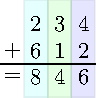
\includegraphics[]{rekfig/plus1}
	\end{figure}
}
}\qquad
\parbox{0.3\linewidth}{
\eks[2]{
	\begin{figure}
		\centering
		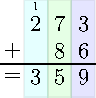
\includegraphics[]{rekfig/plus2}
	\end{figure}
}
}\\[12pt]
\parbox{0.3\linewidth}{
\eks[3]{
	\begin{figure}
		\centering
		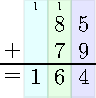
\includegraphics[]{rekfig/plus3}
	\end{figure}
}}\qquad
\parbox{0.3\linewidth}{
\eks[4]{
	\begin{figure}
		\centering
		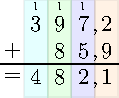
\includegraphics[]{rekfig/plus4}
	\end{figure}
}}
\end{center}
\fork{Example 1}{
\begin{figure}
	\centering
	\subfloat[]{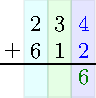
\includegraphics{rekfig/plus1a}}\qquad
	\subfloat[]{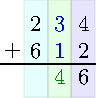
\includegraphics{rekfig/plus1b}}\qquad
	\subfloat[]{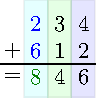
\includegraphics{rekfig/plus1c}}
\end{figure}

\begin{enumerate}[label=\alph*)]
	\item We add the ones: $ 4+2=6 $
	\item We add the tens: $ 3+1=4 $
	\item We add the hundreds: $ 2+6=8 $
\end{enumerate}
} \newpage
\fork{Example 2}{
	\begin{figure}
		\centering
		\subfloat[]{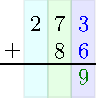
\includegraphics{rekfig/plus2a}}\qquad
		\subfloat[]{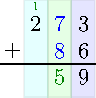
\includegraphics{rekfig/plus2b}}\qquad
		\subfloat[]{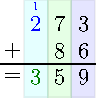
\includegraphics{rekfig/plus2c}}
	\end{figure}
	
	\begin{enumerate}[label=\alph*)]
		\item We add the ones: $ 3+6=9 $
		\item We add the tens: $ {7+8=15} $. Since 10 tens equals 100, we add 1 to the hundreds position, and write the remaining 5 tens at the tens position.
		\item We add the hundreds: $ 1+2=3 $.
	\end{enumerate}
} \vsk

\spr{
Writing 1 on a place value to the left is calle ''carrying 1 over''.
}
\begin{comment}
	\subsubsection{The table method}
	This method starts with one of the terms and add numbers until the other term is reached. You are free to chose which numbers to add as long as you don't exceed the term you are supposed to reach.
	\begin{center}
		\parbox{0.3\linewidth}{
			\eks[1]{
				$ \colb{273}+\colc{86} = \colo{359} $ \vsk
				
				\begin{tabular}{r|r|r}
					&&\colb{273} \\ \hline
					6 & 6 & 279 \\
					30& 36 & 309 \\
					50& \colc{86} & \colo{359}
				\end{tabular}
			}
		} \qquad
		\parbox{0.3\linewidth}{
			\eks[2]{
				$ \colb{85}+\colc{79}=\colo{164} $  \vsk
				
				\begin{tabular}{r|r|r}
					& & \colb{85} \\ \hline 
					5 & 5 & 90 \\
					10 & 15 &100 \\
					64 & \colc{79} & \colo{164} \\
				\end{tabular} \vsk
			}
		}
	\end{center}
	\newpage
	\fork{Example 1}{
		\begin{figure}
			\centering
			\subfloat[]{
				\begin{tabular}{r|r|r}
					&&\colb{273} \\ \hline
					&  &  \\
					\phantom{30}& \phantom{36} &  \\
					&  & 
				\end{tabular}
			} \qquad
			\subfloat[]{
				\begin{tabular}{r|r|r}
					&&\colb{273} \\ \hline
					6& 6 & 279 \\
					\phantom{30}& \phantom{36} &  \\
					&  & 
				\end{tabular}
			}\vsk 
			
			\subfloat[]{
				\begin{tabular}{r|r|r}
					&&\colb{273} \\ \hline
					6& 6 & 279 \\
					30& 36 & 309  \\
					&  & 
				\end{tabular}
			}
			\qquad
			\subfloat[]{
				\begin{tabular}{r|r|r}
					&&\colb{273} \\ \hline
					6& 6 & 279 \\
					30& 36 & 309  \\
					50& \colc{86} & \colo{359}
				\end{tabular}
			}
		\end{figure}
		\begin{enumerate}[label=(\alph*)]
			\item We start with one of the terms. Often, it's wise choose the larger term.
			\item We add $ 6 $. In total we have added $ 6 $, and $ {273+6=279} $.
			\item We add 30. In total we have added 36, and $ 279+30=309 $.
			\item We add 50. In total we have added 86, which is our other term. Moreover, $ 309+50=359 $.
		\end{enumerate}
	} \vsk
	
	\info{Column addition versus the table method}{
		At first sight, the table method may seem like a somewhat cumbersome way of calculating addition. However, the flexibility it showcases when it comes to choosing numbers can be utilized when performing mental arithmetic. But the real strengths of the table method are most apparent when it comes to performing subtraction and division.
	}
\end{comment}

\section{Subtraction}
\subsubsection{Column subtraction}
This method is founded on the base-10 positional notation, in turn subtracting the ones, the tens, the hundreds and so on. It is also based on the perspective of numbers as amounts, so it does not allow negative differences. (see the explanation of \textsl{Example 2}).
\begin{center}
	\parbox{0.3\linewidth}{
\eks[1]{
	\begin{figure}
		\centering
		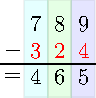
\includegraphics[]{rekfig/min1}
	\end{figure}
}} \qquad
\parbox{0.3\linewidth}{
\eks[2]{
	\begin{figure}
		\centering
		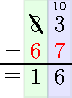
\includegraphics[]{rekfig/min2}
	\end{figure}
}} \\[12pt]
\parbox{0.3\linewidth}{
\eks[3]{
	\begin{figure}
		\centering
		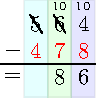
\includegraphics[]{rekfig/min3}
	\end{figure}
}}\qquad
\parbox{0.3\linewidth}{
\eks[4]{
	\begin{figure}
		\centering
		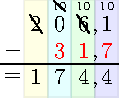
\includegraphics[]{rekfig/min4}
	\end{figure}
}}

\end{center}
\fork{Example 1}{ \vs
\begin{figure}
	\centering
	\subfloat[]{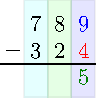
\includegraphics{rekfig/min1a}}\qquad
	\subfloat[]{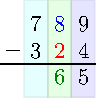
\includegraphics{rekfig/min1b}}\qquad
	\subfloat[]{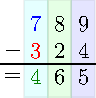
\includegraphics{rekfig/min1c}}
\end{figure}

\begin{enumerate}[label=(\alph*)]
	\item We find the difference between the ones: $ {9-4=5} $
	\item We find the difference between the tens: $ {8-2=6} $. 
	\item We find the difference between the hundreds: $ {7-3=4} $.
\end{enumerate}
}
\newpage
\fork{Example 2}{ \vs
	\begin{figure}
		\centering
		\subfloat[]{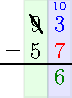
\includegraphics{rekfig/min2a}}\qquad
		\subfloat[]{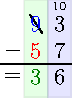
\includegraphics{rekfig/min2b}}
	\end{figure}
	
	\begin{enumerate}[label=(\alph*)]
		\item We notice that 7 is larger than 3, and thus we take 1 ten from the 9 at the tens position. This is marked by drawing a line across 9. Then we find the difference between the ones: $ {13-7=6} $
		\item Since we took 1 from the 9 tens, it is now only 8 tens. We find the difference between the tens: $ {8-5=3} $.
	\end{enumerate}
}
\subsubsection{The table method}
The table method takes advantage of subtraction being the inverse operation of addition. For example, the answer to the question ''What is $ 789-324 $?'' is the same as the answer to the question ''How much must i add to 324 in order to get 789?''. With the table method you can freely chose which numbers to add as long as you end up with the targeted number.\\
\begin{center}
\parbox{0.35\linewidth}{
\eks[1]{
$ \colb{789}-\colr{324}=\colc{465} $	 \vsk

\begin{tabular}{r|r}
	& \colr{324} \\ \hline
	6&330 \\
	70&400 \\
	389&\colb{789} \\ \hline
	\colc{465}
\end{tabular}
}} \qquad
\parbox{0.35\linewidth}{
	\eks[2]{
		$ \colb{83}-\colr{67}=\colc{16} $	 \vsk
		
		\begin{tabular}{r|r}
			& \colr{67} \\ \hline
			3&70 \\
			13&\colb{83} \\ \hline
			\colc{16}
		\end{tabular} \vspace{14pt}
}} \\[12pt]
\parbox{0.35\linewidth}{
	\eks[3]{
		$ 564-478=86 $\vsk
		
		\begin{tabular}{r|r}
			& 478 \\ \hline
			2&480 \\
			20&500 \\ 
			64&564\\ \hline
			86
		\end{tabular}
}} \qquad 
\parbox{0.4\linewidth}{
	\eks[4]{
		$ {206,1-31,7=174,4} $\vsk
		
		\begin{tabular}{r|r}
			& 31,7 \\ \hline
			0,3& 32\phantom{,0} \\
			70\phantom{,0}&102\phantom{,0} \\ 
			104,1&206,1\\ \hline
			174,4
		\end{tabular}
}}
\end{center}
\fork{Example 1}{
	\[ \colb{789}-\colr{324}=\colo{465} \]
\begin{figure}
	\centering
	\subfloat[]{
	\begin{tabular}{r|r}
		& \colr{324} \\ \hline
		& \\
		& \\
		& \\ \hline
		&
	\end{tabular}	
} \qquad
	\subfloat[]{
	\begin{tabular}{r|r}
		& \colb{324} \\ \hline
	   \colb{6}& \colc{330}\\
		& \\
		& \\ \hline
		&
	\end{tabular}
}\qquad
	\subfloat[]{
	\begin{tabular}{r|r}
		& 324 \\ \hline
		6& \colb{330}\\
		\colb{70}& \colc{400} \\
		& \\ \hline
		&
	\end{tabular}	
}  \\[12pt]
\subfloat[]{
	\begin{tabular}{r|r}
		& 324 \\ \hline
		6& 330\\
		70& \colb{400} \\
		\colb{389}& \colc{789}\\ \hline
		&
	\end{tabular}	
}\qquad
\subfloat[]{
	\begin{tabular}{r|r}
		& 324 \\ \hline
		\colb{6}& 330\\
		\colb{70}& 400 \\
		\colb{389}& 789\\ \hline
		\colo{465}&
	\end{tabular}	
}
\end{figure}
\begin{enumerate}[label=(\alph*)]
	\item We start at 324.
	\item We add 6, and get $ {324+6=330} $
	\item We add 70, and get $ {70+330=400} $
	\item We add 389, and get $ {389+400=789} $. Now we have reached 789.
	\item We find the sum of the numbers we added: $ {6+70+389=465} $
\end{enumerate}
}
\section{Multiplication} \label{rekGanging}
\subsubsection{Multiplying by 10, 100, 1\,000 etc.}
\reg[Å gange heltall med 10, 100 osv. \label{gangheltallmed10100}]{
	\vs
	\begin{itemize}
		\item When multiplying an integer by 10, the product can be found by adding the digit 0 behind the integer.
		\item When multiplying an integer by 100, the product can be found by adding the digits 00 behind the integer.
		\item The same pattern applies for the numbers 1\,000, 10\,000 etc.
	\end{itemize}
}
\eks[1]{\vsb \vsb
	\alg{
		6\cdot \colb{10} &= 6\colb{0}\vn
		79\cdot \colb{10} &= 79\colb{0} \vn
		802\cdot\colb{10}&=802\colb{0}
	}
}
\eks[2]{ \vsb \vsb
\alg{ 
6\cdot\colb{100} &= 6\colb{00} \vn
79\cdot\colb{100} &= 7\,9\colb{00} \vn
802\cdot\colb{100} &=80\,2\colb{00}
}
}
\eks[3]{ \vsb \vsb
\alg{ 
	6\cdot\colb{1\,000} &= 6\,\colb{000} \vn
	79\cdot\colb{10\,000} &= 79\colb{0\,000} \vn
	802\cdot\colb{100\,000} &=80\,2\colb{00\,000}
}
}
\newpage
\reg[Multiplying decimal numbers by 10, 100, etc. \label{gangdesmed10100}]{
	\vs
	\begin{itemize}
		\item When multiplying a decimal number by 10, the product is found by moving the dot one position to the right. 
		\item When multiplying a decimal number by 100, the product is found by moving the dot one position to the right.
		\item The same pattern applies for the numbers 1\,000, 10\,000 etc.
	\end{itemize}
}
\eks[1]{\vsb \vsb
	\alg{
		7\colr{.}9\cdot 10 &= 79\colr{.}=79 \vn
		38\colr{.}02\cdot10&=380\colr{.}2 \vn
		0\colr{.}57\cdot 10 &=05\colr{.}7=5\colr{.}7 \vn
		0\colr{.}194\cdot 10&= 01\colr{.}94=1\colr{.}94
	}
}
\eks[2]{ \vsb \vsb
	\alg{
		7\colr{.}9\cdot 100 &= 790\colr{.}=790 \vn
		38\colr{.}02\cdot100&=3802\colr{.}=3\,802 \vn
		0\colr{.}57\cdot 100 &=057\colr{.}=57 \vn
		0\colr{.}194\cdot 100&= 019\colr{.}4=19\colr{.}4
	}
}
\eks[3]{ \vsb \vsb
	\alg{
	7\colr{.}9\cdot 1\,000 &= 7900\colr{.}=7\,900 \vn
	38\colr{.}02\cdot10\,000&=380020\colr{.}=380\,200 \vn
	0\colr{.}57\cdot 100\,000 &=57000\colr{.}=57\,000
}
}
\info{\note}{
\hrs{gangheltallmed10100}{Rule} is just a special case of \rref{gangdesmed10100}. For example, applying \rref{gangheltallmed10100} when calculating $ {7\cdot 10} $ yields the same answer as when applying \rref{gangdesmed10100} when calculating $ {7,0\cdot 10} $. 
}
\newpage
\fork{Multiplying by 10, 100 etc.}{
The Base-10 positional notation is founded on groups of tens, hundreds, thousands etc., and tenths, hundredths, thousandths etc. (see \rref{titalsys}). When multiplying a number by 10, all the ones in the number will form a group of tens, all the tens will form a group of hundreds an so on. Hence, every digit is moved one position to the left. Similarly, every digit is moved one position to the left when multiplying by 100, three places when multiplying by 1\,000 etc.
}
\subsubsection{Expanded form}
Multiplication with expanded form can be applied on multi digit numbers. The method is based on the distributive law (\rref{gangpar}). \regv
\eks[1]{ \vs
\begin{figure}
	\centering
	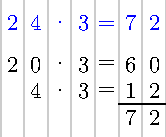
\includegraphics[]{rekfig/gang1}
\end{figure}
}
\eks[2]{ \vs
\begin{figure}
	\centering
	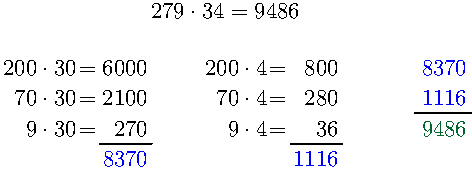
\includegraphics[]{rekfig/gfleirsif}
\end{figure}
}
\fork{Example 1}{
24 can be written as $ 20+4 $, so
\[ 24\cdot3 =(20+4)\cdot3 \]
Moreover, by \rref{gangpar},
\alg{
(20+4)\cdot 3 &=20\cdot 3 + 4\cdot 3 \\
&= 60+12 \\
&= 72
}
}
\newpage
\fork{Example 2}{
We have
\algv{
279&=200+70+9 \\
34 &=30+4 	
}
Thus
\[ 279\cdot34= (200+70+9)\cdot (30+4) \]
Moreover,
{
\footnotesize
\alg{
(200+70+9)\cdot (30+4) &=200\cdot 30+70\cdot30+9\cdot30+200\cdot4+70\cdot4+9\cdot4
\\
&=9486}
} \vs
}
\subsubsection{The compact method}
The compact method is based on the same principles as the expanded form method, only with a shorter way of writing. \regv

\eks[1]{
	\begin{figure}
		\centering
		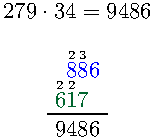
\includegraphics[]{rekfig/gfleirsifa}
	\end{figure}
}
\newpage
\fork{Example 1}{
First we multiply the digits of 279 by 4:
\begin{itemize}
	\item $ 9\cdot 6=36 $, so we write 6 at the ones position and carry\\ over 3.
	\item $ 7\cdot4 =28$, so we write 8 at the tens position and carry\\ over 2.
	\item $ 2\cdot 4=8 $, so we write 8 at the hundreds position.
\end{itemize}
Then we multiply the digits of 279 by 30. This in turn can be simplified to multiplying by 3, as long as we shift the digits one position to the left, relative to when we multiplied by 4:
\begin{itemize}
	\item $ 9\cdot 3=27 $, so we write 7 at the tens position and carry \\ over 2. 
	\item $ 7\cdot3=21 $, so we write 1 at the hundreds position and carry \\ over 2.
	\item $ 2\cdot3=6 $, so we write 6 at the thousands position.
\end{itemize} 
}
\section{Division} \label{rekDivisjon}
\subsubsection{Division by 10, 100, 1\,000 etc.}
\reg[Deling med 10, 100, 1\,000 osv. \label{deledesmed10100}]{
When dividing a decimal number by 10, the quotient is found by moving the dot one position to the left.\vsk

When dividing a decimal number by 100, the quotient is found by moving the dot two positions to the left.\vsk

The same pattern applies for the numbers 1\,000, 10\,000 etc.
}
\eks[1]{ \vsb \vsb
	\alg{
200:10&=200\colr{.}0:10 \\&=20\colr{.}00\\&=20	\vn
45:10&=45\colr{.}0:10 \\&= 4\colr{.}50 \\&=4\colr{.}5
}
}
\eks[2]{ \vsb \vsb
	\alg{
		200:100&=200\colr{.}0:100 \\&=2\colr{.}000\\&=2	\vn
		45:100&=45\colr{.}0:100 \\&= 0\colr{.}450 \\&=0\colr{.}45
	}
}
\newpage
\eks[3]{ \vsb \vsb
\alg{
143\colr{.}7 :10 &= 14\colr{.}37 \vn
143\colr{.}7 :100 &= 1\colr{.}437 \vn
143\colr{.}7 :1\,000 &= 0\colr{.}1437 
}
}
\eks[4]{ \vsb \vsb
\alg{
93\colr{.}6:10 &= 9\colr{.}36 \vn
93\colr{.}6:100 &= 0\colr{.}936 \vn
93\colr{.}6:1\,000 &= 0\colr{.}0936
}
}
\fork{Division by 10, 100, 1\,000 osv.}{
The Base-10 positional notation is founded on groups of tens, hundreds, thousands etc., and tenths, hundredths, thousandths etc. (see \rref{titalsys}). When dividing a number by 10, all the ones in the number will form a group of tens, all the tens will form a group of ones an so on. Hence, every digit is moved one position to the right. Similarly, every digit is moved two positions to the right when multiplying by 100, three places when multiplying by 1\,000 etc.
}

\subsubsection{Long division}
Long division is based on the perspective of numbers as amount (see page \pageref{Divisjon}).

\begin{center}
	\parbox{0.3\linewidth}{
	\eks[1]{ \vsb
		\begin{figure}
			\centering
			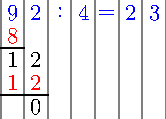
\includegraphics[]{rekfig/del1}
		\end{figure} \vspace{18pt}
	}
}\qquad
\parbox{0.45\linewidth}{
	\eks[1]{ \vspace{-5pt}
		\begin{figure}
			\centering
			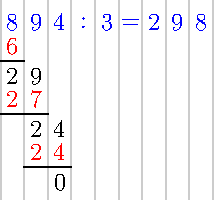
\includegraphics[]{rekfig/del2}
		\end{figure}
	}
}
\end{center}
\newpage
\fork{Example 1}{ \vs \vs
	\begin{figure}
		\centering
		\subfloat{\includegraphics{\figp{delalg}}}
		\qquad \subfloat{\includegraphics[angle=90]{\figp{delalg0}}}
	\end{figure}
	The above figure illustrates the amount 92, which we shall divide into 4 equal groups. 
	\begin{itemize}
		\item We start by distributing as many tens as possible. Of the 9 tens, each group can get 2. In total we have distributed $ 2\cdot 4=8 $ tens.
		\begin{figure}
			\centering
			\subfloat{\includegraphics{\figp{delalgaa}}}
			\qquad \subfloat{\includegraphics[angle=90]{\figp{delalga}}}
		\end{figure}
		\item Now we are left with 1 ten and 2 ones, which equals 12 ones. Of the 12 ones, each group can get 3. In total we have distributed $ 3\cdot 4= 12 $ ones.
		\begin{figure}
			\centering
			\includegraphics[angle=90]{\figp{delalgb}}
		\end{figure}
		\item The amount we started with, 92, is now equally distributed, and our calculation is done. In each group we got 23.
	\end{itemize}
}
\newpage
\subsubsection{The table method}
The table method takes advantage of division being the inverse operation of multiplication. For example, the answer to the question ''What is $ {76:4} $?'' is the same as the answer to the question ''Which number yields 76 when multiplied by 4?''. In the same way as with the table method for subtraction, the numbers can be chosen more ore less freely.
\begin{center}
	\label{ekstbldiv}
	\parbox{0.35\linewidth}{
		\eks[1]{
			$ \colg{92}:\colb{4}=\colo{23} $	 \vsk
			
			\begin{tabular}{r|r|r}
				$ \cdot\, \colb{4} $&\\ \hline
				10&40&40 \\
				10&40&80 \\
				3& 12 &\colg{92} \\ \hline
				\colo{23}&
			\end{tabular}
			\vspace{28pt}
		}} \qquad
\parbox{0.35\linewidth}{
	\eks[2]{
		$ \colg{894}:\colb{3}=\colo{298} $	 \vsk
		
		\begin{tabular}{r|r|r}
			$ \cdot\, \colb{3} $&\\ \hline
			200& 600 &600 \\
			30&90 &690 \\
			30&90 &780 \\
			30& 90&870 \\
			8&24 &\colg{894} \\ \hline
			\colo{298} &
		\end{tabular}
}} \vsk

\parbox{0.415\linewidth}{
	\eks[3]{		
		$ 894:3=298 $	 \vsk
		
		\begin{tabular}{r|r|r}
			$ \cdot\, 3 $&\\ \hline
			300& 900&900 \\
			$ -2 $& $ -6 $ &894 \\ \hline
			298&
		\end{tabular} \vsk
	
\footnotesize	
\notesm{Same task as in \textsl{Example 2} but a different calculation.} 
}
}
\end{center}
\newpage
\fork{Example 1}{
	Since we are to divide \colg{92} by \colb{4}, we multiply numbers by \colb{4} until we reach \colg{92}.
	\begin{figure}
		\centering
		\subfloat[]{
			\begin{tabular}{r|r|r}
				$ \cdot\, \colb{4} $&\\ \hline
				10&40&40 \\
				&& \\
				& &\\ \hline
				&
			\end{tabular}	
		} \qquad
		\subfloat[]{
			\begin{tabular}{r|r|r}
				$ \cdot\, \colb{4} $&\\ \hline
				10&40&40 \\
				10&40&80 \\
				&  & \\ \hline
				&
			\end{tabular}	
		} \\
		\subfloat[]{
			\begin{tabular}{r|r|r}
				$ \cdot\, \colb{4} $&\\ \hline
				10&40&40 \\
				10&40&80 \\
				3& 12 &\colg{92} \\ \hline
				&
			\end{tabular}	
		} \qquad
		\subfloat[]{
			\begin{tabular}{r|r|r}
				$ \cdot\, \colb{4} $&\\ \hline
				10&40&40 \\
				10&40&80 \\
				3& 12 &\colg{92} \\ \hline
				\colo{23}&
			\end{tabular}	
		}
	\end{figure}
	\begin{enumerate}[label=(\alph*)]
		\item We multiply 10 by 4, which equals 40. So far we have reached 40.
		\item We multiply 10 by 4, which equals 40. So far we have reached $ {40+40=80} $.
		\item We multiply 3 by 4, which equals 12. So far we have reached $ {80+12=92} $, which was our target.
		\item We add the numbers we multiplied by 4: $ {10+10+3=23} $.
	\end{enumerate}
}\vsk

\info{Tip}{
	It is wise to look back at calculations done with the table method and search for improvements. In \textsl{Example 1} on page \pageref{ekstbldiv}, we could have started off multiplying by 20. This is almost as easy as multiplying by 10, and it takes us closer to the target.
}
\newpage
\subsubsection{Divisjon med rest}
The value of a division calculation is far from always an integer. One way of expressing the answer is by using the term \outl{remainder}\index{remainder}. What it means is best explained through an example: \regv
\eks[1]{
	Calculate $ 11:4 $ using remainder.
	
	\sv
	The largest integer we can multiply by 4 without having a product exceeding 11 is 2. $ {2\cdot 4 = 8} $, so we have ${ 11-8=3 }$ left to reach 11.
	\[ 11= \colb{2}\cdot 4 +\colc{3} \]	
	\fig{mod1}
	This means that
	\[ 11:4 =\text{\colb{2} and \colc{3} in remainder}\]
}
\eks[2]{
	Calculate $ 19:3 $ using remainder.
	
	\sv
	The largest integer we can multiply by 3 without exceeding 19 is 6. $ {6\cdot 3 = 18} $, so we have $ 19-8=1 $ left to reach 19.
	\[ 19= \colb{6}\cdot 3 +\colc{1} \]	
	\fig{mod2}
	This means that
	\[ 19:3 =\text{\colb{6} and \colc{1} in remainder}\]
}
\newpage
\eks[3]{
	Calculate $ 94:4 $ using remainder.
	
	\sv
	\metode{Using long division}{3.75cm}
	\[ 94:4 = \text{23 og 2 i rest} \]
	\begin{figure}
		\centering
		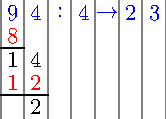
\includegraphics[]{rekfig/mod3}
	\end{figure}
	\notesm{Since it's wrong to use \sym{$ = $} in the above calculation, we have chosen to use \sym{$  \rightarrow$}. 
	}\vsk 
	
	\metode{Using the table method}{3.75cm}
	\[ 94:4 = \text{23 and 2 in remainder} \]
	\begin{center}
		\begin{tabular}{r|r|r}
			$ \cdot\, 4$&\\ \hline
			20&80&80 \\
			3& 12 &92 \\ \hline
			23&
		\end{tabular} \qquad $ 94-92=2 $
	\end{center}
} \vsk

\spr{
	Performing a \outl{modulo-operation}, we find the remainder of a division calculation. This is often abbreviated as \sym{mod}. For example is
	\[ 11\text{ mod } 4= 3\qquad , \qquad 19\text{ mod 3} =1 \]
	In addition to \sym{\texttt{mod}}, \sym{\texttt{\%}} and \sym{{\texttt{\string //}}} are common symbols for this operation in programming languages.
}
\newpage
\subsubsection{Divisjon using mixed numbers}
\eks[1]{
	Calculate $ 11:4 $ using mixed numbers.
	
	\sv \vsb
	\[ 11:4 = \text{2 and 3 as remainder}=2+\frac{3}{4} \]
}
\eks[2]{
	Calculate $ 19:3 $ using mixed numbers.
	
	\sv \vsb
	\[ 19:3=\text{6 and 1 in remainder}=6+\frac{1}{3} \]
} \vsk

\fork{Example 1}{
	We start by noticing that $ 4=\frac{4}{1} $. Hence
	\[ 11:4 = 11:\frac{4}{1} \]
	From \rref{delmbr} it follows that
	\[ 11:\frac{4}{1} = 11\cdot \frac{1}{4} \]
	Moreover, $ 11=2\cdot 4+ 3 $, and thus
	\[ 11\cdot \frac{1}{4}=(2\cdot 4+3)\cdot\frac{1}{4} \]
	Now, by \rref{gangpar},
	\alg{
		(2\cdot 4+3)\cdot\frac{1}{4}&=2\cdot4\cdot\frac{1}{4}+3\cdot \frac{1}{4} \\
		&= 2+\frac{3}{4}
	}
}
\newpage
\subsection{Division using decimal numbers}
\eks[1]{
	Calculate $ 11:4 $ using a decimal number.
	
	\sv
	
	\metode{With long divsion}{3.75cm} \vs
	\[ 11:4=2,75 \]
	\begin{figure}
		\centering
		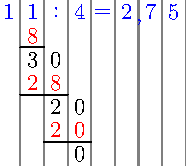
\includegraphics{rekfig/deldes1}
	\end{figure}
	\metode{With the table method}{3.75cm} \vs
	\[ 11:4 = 2,75\]
	\begin{center}
		\begin{tabular}{r|r|r}
			$ \cdot\, 4$&\\ \hline
			2&8&8 \\
			0,5& 2 &10 \\
			0,25& 1 &11\\ \hline
			2,75&
		\end{tabular}
	\end{center}
}
\fork{Example 1; long division}{
	Since we divide 4, we seperate 11 in 4 equal groups.
	\begin{itemize}
		\item We can equally distribute 8 of the 11 ones in 4 groups. Then there are 3 ones left. This equals 30 tenths.
		\item 28 of the 30 tenths can be equally distributed in 4 groups. Then there are 2 tenths left. This equals 20 hundredths.
		\item 20 of the 20 hundredths can be equally distributed in 4 groups.
		\item Now the whole amount of 11 is equally distributed, so our calculation is finished.
	\end{itemize}
}
\newpage
\section{Calculation with time \label{regningmedtid}}
Seconds, minutes and hours are organized in groups of 60:
\alg{
	1\text{ minute} &= 60\text{ second} \\
	1\text{ hour} &= 60\text{ minute} 
}
This means that \textsl{crossovers} arise in the calculations when we reach 60.\regv

\eks[1]{
	$ \text{2\enh{h} 25\enh{min} } + \text{10\enh{h} 45\enh{min}}= \text{13\enh{h} 10\enh{min} } $\vsk
	
	\metode{Method 1}{0.35\linewidth}
	\os
	\begin{tabular}{r|r|r}
		& &10\enh{h} 45\enh{min}  \\ \hline
		15\enh{min}  &15\enh{min} & 11\enh{h} 00\enh{min}  \\
		10\enh{min} &25\enh{min} & 11\enh{h} 10\enh{min} \\
		2\enh{h} & 2\enh{h} 25\enh{min}  & 13\enh{h} 10\enh{min}
	\end{tabular} \vsk \vsk
	
	\metode{Method 2}{0.35\linewidth}\os
	\begin{tabular}{r|r|r}
		& & 10:45 \\ \hline 
		00:15 & 00:15 & 11:00 \\
		00:10 & 00:25 & 11:10 \\
		02:00 & 02:25 & 13:10
	\end{tabular}
} \regv

\eks[2]{
	$ \text{14\enh{h} 18\enh{min} } - \text{9\enh{h} 34\enh{min}}= \text{4\enh{h} 44\enh{min} } $\vsk
	
	\begin{center}
		\parbox{0.4\linewidth}{
			\metode{Method 1}{0.9\linewidth} \os
			\begin{tabular}{r|r}
				&  9\enh{h} 34\enh{min} \\ \hline 
				26\enh{min} & 10\enh{h} 00\enh{min} \\
				18\enh{min} & 10\enh{h} 18\enh{min} \\
				4\enh{h} & 14\enh{h} 00\enh{min} \\ \hline
				4\enh{h} 44\enh{min}
			\end{tabular}
		} \qquad \qquad
		\parbox{0.4\linewidth}{
			\metode{Method 2}{0.9\linewidth} \os
			\begin{tabular}{r|r}
				& 09:34 \\ \hline 
				00:26 & 10:00 \\
				00:18& 10:18 \\
				04:00 & 14:18 \\ \hline
				04:44 
			\end{tabular}
		}
	\end{center}
}


\section{Rounding and estimates}

\subsubsection{Rounding}
When \outl{rounding}, we decrease the amounts of digits other than 0 in a number. Also, we can round off to the \textsl{closest one}, \textsl{the closest ten} and such.\regv
\eks[1]{
	When rounding off to the \textsl{closest ten} we round off
	\begin{itemize}
		\item 1, 2, 3 and 4 \textsl{down} to 0, because they are closer to 0 than to 10.
		\item 6, 7, 8 and 9 \textsl{up} to 10 because they are closer to 10 than to 0.
	\end{itemize}	
	5 avrundes også opp til 10.
	\fig{avrnd0}
}

\eks[2]{ \vs
	\begin{itemize}
		\item $\boldmath \textbf{63 rounded off the the closest 10} = 60 $ \\
		Because 63 is closer to 60 than 70.
		\fig{avrnda}
		\item $\boldmath \textbf{78 rounded off to the closest ten} = 80 $ \\
		Because 78 is closer to 80 than 70.
		\fig{avrndb}
		\item $\boldmath \textbf{359 rounded off to the closest hundred} = 400 $\\
		Because 359 is closer to 400 than 300.
		\fig{avrndc}
		\item $ \boldmath \textbf{11,8 rounded off to the closest one} = 12$ \\
		Because 11,8 is closer to 12 than 11.
		\fig{avrndd}
	\end{itemize}
}

\subsection{Estimate}
Rather than knowing the exact answer to a calculation, at times there is more important to quickly determine the outcome \textsl{approximately}, preferably by mental arithmetic. When finding an approximate answer, the result is called an \outl{estimate}. An estimate involves rounding off\footnote{Note: Rounding off when performing estimates does not necessarily involve rounding off to the closes one, ten or such.} numbers so that the calculation is easier to perform. \regv

\spr{
	That something is ''about the same as'' is often written as ''cirka'' (''ca.''). The symbol for ''cirka'' is \sym{$ \approx $}.
} 

\subsubsection{Estimates when adding or multiplying}
Let us estimate the calculation
\[ 98.2+24.6 \]
We have $ 98,2 \approx 100 $. If we write 100 instead of 98.2 in our calculation, the result will slightly exceed the exact answer. Therefore, if we are to round off 24.6 we should round it off downwards. 24.6 is pretty close to 20, we can write
\[ 98.2+24.6 \approx 100 + 20 = 120 \]
As this example showcases, when making an estimate involving addition, we should try to round off one of the numbers (upwards) and the other number (downwards).\\

\linje
The same applies for estimates involving multiplication. Let us\\ estimate
\[ 1\,689\cdot12 \]
We round off 12 to 10. In that case, the estimate will result in an answer lower than the exact anser, so to account for this we round off 1\,689 uo to 1\,700. Now
\[ 1\,689\cdot12\approx 1\,700\cdot 10 =17\,000 \]
\subsubsection{Estimation when subtracting and dividing}
Let us make an estimate of
\[ 186,4-28,9 \]
If we round off 186,4 up to 190, the result will be slightly larger than the exact answer. To account for this, we should subtract a bit more than in the original calculation. That can be done by rounding off 28,9 up (to 30):
\alg{
	186.4-28,9&\approx 190-30 \\&=160
}
\linje
The same principle applies when an estimate involves division. Let us estimate
\[ 145:17 \]
We round off 17 up to 20. This will make our result a bit smaller than the exact answer. Hence, we should also round off 145 upwards (to 150):
\[ 145:17 \approx 150:20 = 75 \]

\subsubsection{Estimation, summary}
\reg[Estimation \label{tipsoverslag}]{ \vs
	\begin{itemize}
		\item Ved addisjon eller multiplikasjon mellom to tall, avrund gjerne et tall opp og et tall ned.
		\item Ved subtraksjon eller deling mellom to tall, avrund gjerne begge tall ned eller begge tall opp.
	\end{itemize}	
}
\newpage
\eks[]{
	Estimate the calculations.\os
	
	\abch{
		\item $ {23,1+174,7} $ 
		\item $ {11,8\cdot107,2} $ 		
	} \os
	\abchs{3}{
		\item $ {37,4-18,9} $  \ \ 
		\item $ {1054:209} $
	}
	\vspace{-2pt}
	
	\sv  \vspace{-7pt}
	\abc{
		\item $ 32,1 + 174,7 \approx 30+170 = 200 $
		\item $ 11.8 \cdot 107.2 \approx 10\cdot110 = 1\,100 $
		\item $ 37.4 - 18.9 \approx 40-20 = 20 $
		\item $ 1\,054:209 \approx 1\,000:200 = 5 $
	}
} \vsk

\info{Comment
}{
	There are no specific rules for what you \textsl{can} or \textsl{can not} do when making an estimate. Thereby, \rref{tipsoverslag} is strictly speaking not a rule but rather a useful tip.\vsk
	
	It is also natural to raise the question how far away from the exact answer an estimate is allowed to be. Neither in this case are there any rules to follow. However, an estimate and the exact answer should have the same \outl{order of magnitude}. Simply put, if the exact answer has something to do with thousands, then so should also the estimate. 
	To be more concise, the exact answer and the estimate shall have the same power of 10 when written in standard form\footnote{See \refsec{Standardform}}.
}
\newpage
\section{Standard form} \label{Standardform}
\textit{Note: In this section it is taken for granted that the reader is familiar with powers, which we study in \refsec{Potensar}.}\vsk

We can apply \rref{gangdesmed10100} and \rref{deledesmed10100}, and what we know about powers, to write numbers in \outl{standard form}. \vsk

Let us look at the number 6\,700. By \rref{gangdesmed10100},
\[ 6\,700=6.7\cdot1\,000 \]
Since $ 1000=10^3 $, we have
\[ 6\,700=6,7\cdot1\,000=6.7\cdot 10^3 \]
\st{
	$ 6.7\cdot10^3 $ er 6\,700 written in standard form because
	\begin{itemize}
		\item 6.7 is larger than or equal to 1, and smaller than 10.
		\item $ 10^3 $ is a power with base 10 and exponent 3, which is an integer.
		\item The product of 6,7 and $ 10^3 $ equals $ 6\,700 $.
	\end{itemize}
}
\linje \\[12pt]

Let us look at the number 0.093. By \rref{deledesmed10100},
\[ 0.093=9.3: 100 \]
Dividing by 100 is the same as multiplying by $ 10^{-2} $, so
\[ 0.093=9.3: 100=9.3\cdot10^{-2} \]
\st{
	$ 9,3\cdot10^{-2} $ is 0,093 written in standard form because
	\begin{itemize}
		\item 9.3 is larger than or equal to 1, and smaller than 10.
		\item $ 10^{-2} $ is a power with base 10 and exponent $ -2 $, which is an integer.
		\item The product of $ 9,3 $ and $ 10^{-2} $ equals 0.093.
	\end{itemize} 
}
\reg[Standardform]{
	A number written on the form
	\[ a\cdot 10^n \]
	where $ {1\leq|a|<10} $ and $ n $ is an integer, is a number written in \outl{standard form}.
}
\eks[1]{
	Write 980 in standard form.
	
	\sv \vsb
	\[ 980 = 9.8\cdot 10^2 \]
}
\eks[2]{
	Write 0.00671 in standardform.
	
	\sv \vsb
	\[ 0.00671 = 6.71\cdot 10^{-3} \]
}\vsk

\info{Tip}{
	To write numbers in standard form you can do the following:
	\begin{enumerate}
		\item Move the decimal separator so that you get a number between 1 and 10.
		\item Multiply this number by a power of ten with exponent equal to the amount of places you moved the decimal separator.  If you moved the decimal seperator to the left/right, the exponent is positive/negative. 
	\end{enumerate}
}
\newpage
\eks[3]{
	Write 9\,761\,432 in standard form.
	
	\sv \vs
	\begin{enumerate}
		\item We move the decimal separator 6 places to the left, and get $ 9\colr{.}761432 $
		\item We multiply this number by $ 10^6 $, and get 
		\[ 9\,761\,432=9.761432\cdot 10^6 \] 
	\end{enumerate}
}
\eks[4]{
	Write 0.00039 in standard form
	
	\sv \vs
	\begin{enumerate}
		\item We move the decimal separator 4 places to the right, and get $ 3,9 $.
		\item We multiply this number by $ 10^{-4} $, and get
		\[ 0,00039=3,9\cdot10^{-4} \]
	\end{enumerate}
}
\end{document}

